\chapter
 [Quantum Networking: Background and Challenges]
 {Quantum Networking:\\Background and Challenges}
\label{chp:background}

\begin{abstract}
Quantum networks are a fundamentally new paradigm of telecommunications, destined to enhance our
classical networking primitives to achieve unprecedented tasks in various areas of
communications and sensing. But how do quantum networks differ from their classical counterpart?
What makes them special, and at the same time challenging to manage? This chapter provides useful
background knowledge on quantum networking and recaps the primary challenges thereof.
\end{abstract}

\note{To be precise, this chapter is extracted from sections 1 (Introduction), 2 (Background on
Quantum Networking) and 3.1 (Challenges) from the \acrshort{qnodeos} paper. There aren't any major
additions.}

\blfootnote{
    This chapter is based on the preprint \citetitle{delledonne_2023_qnodeos} by
    \textcite{delledonne_2023_qnodeos}, submitted for peer review.
}

\newpage

% * Quantum networking basics, state of the art, ad-hoc experiments, and (lack of) sophisticated
%   control systems above the physical layer.
% * Recap of what exists for classical networking, including communication protocols, network OSes,
%   SDNs, and what we can learn from these for quantum networking.
% * Limitations of quantum theory and hardware that need addressing when designing abstractions, and
%   generic requirements for such abstractions.

\lettrine{U}{biquitous} internet connectivity has already unlocked a plethora of applications that
were not even conceived just years ago. Similarly, a future quantum
internet~\cite{kimble_2008_quantum, wehner_2018_stages} aims to connect quantum devices --- the
\emph{end nodes}~\cite{wehner_2018_stages} --- over large distances, in order provide new internet
functionality that is impossible to achieve using solely classical communication. Examples of
applications~\cite{wehner_2018_stages} running on end nodes include security-enhancing protocols
such as \acrfull{qkd}~\cite{ekert_1991_e91, bennett_2014_bb84}, improved clock
synchronization~\cite{komar_2014_clocks}, support for distributed
sensing~\cite{gottesman_2012_telescope} and distributed systems~\cite{benor_2005_byzantine}, as well
as secure quantum computing in the cloud~\cite{broadbent_2009_ubqc, childs_2005_secure_qc}.

To run a general quantum networking application, the end nodes' hardware-software system needs to be
capable of performing certain actions, as summarized in \cref{fig:quantum-internet}. First, the end
nodes must be able to establish a quantum connection by generating quantum \emph{entanglement}
between them. Entanglement is a special property of at least two quantum bits --- or \emph{qubits}
--- one held by each end node. The entangled qubits are often measured directly by the application,
or may be used to transmit data qubits from one end node to the other through
teleportation~\cite{bennett_1993_teleportation}. Alongside entanglement, end nodes must be capable
of executing local quantum operations on the qubits held by an end node, that is, quantum
\emph{gates} and quantum \emph{measurements}. For simple quantum applications such as secure
communication~\cite{ekert_1991_e91, bennett_2014_bb84} it is sufficient to produce entanglement and
then perform a local measurement at each end node. However, for more complex quantum applications
--- enabled at higher stages of quantum internet development~\cite{wehner_2018_stages} --- local
operations can include the execution of quantum gates and in fact full quantum computation on a
quantum processor. Finally, next to such quantum actions, most quantum applications known to date
require local classical processing, as well as classical communication between the end nodes.

\begin{figure}[H]
    \begin{center}
        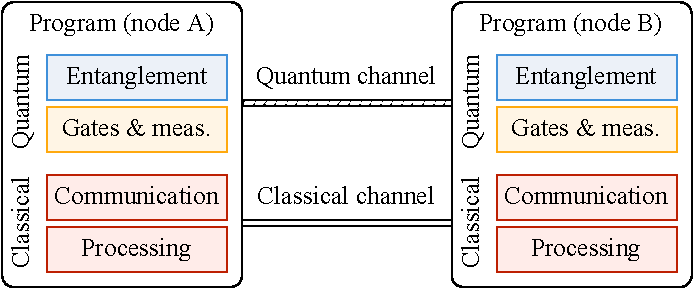
\includegraphics[width=0.6\linewidth]{figures/quantum-internet.pdf}
    \end{center}
    \caption{
        A quantum networking application consists of separate programs running at two or more end
        nodes that communicate via classical message passing and quantum entanglement. Local
        operations include quantum operations (gates and measurements) as well as classical
        processing.
    }
    \label{fig:quantum-internet}
\end{figure}

Abstractly, a quantum networking application consists of multiple programs, each running at one of
the end nodes. The distinct programs only interact with one another by means of entanglement
generation and classical communication. This allows a programmer to realize security sensitive
applications just as in the classical domain, but prohibits a global orchestration of the quantum
execution as one might do in quantum computing. The case of secure quantum computing in the
cloud~\cite{broadbent_2009_ubqc, childs_2005_secure_qc} provides a simple illustrative use case of a
quantum networking application, schematically depicted in \cref{fig:app-struct}. In blind quantum
computing, a client node wants to perform a computation on a remote server node, the latter being a
powerful quantum computer, without the server learning anything about the computation. Blind quantum
computing illustrates the need for a continuing interaction between the classical and quantum parts
of the execution, such as waiting for a message from a remote client before continuing the quantum
execution at the server. It also highlights the need for both classical and quantum state to be kept
alive, for example such that future quantum instructions can be executed depending on messages from
remote end nodes. This is in sharp contrast to quantum computing applications, where one can process
the entire quantum execution in a single batch.

\begin{figure}
    \centering
    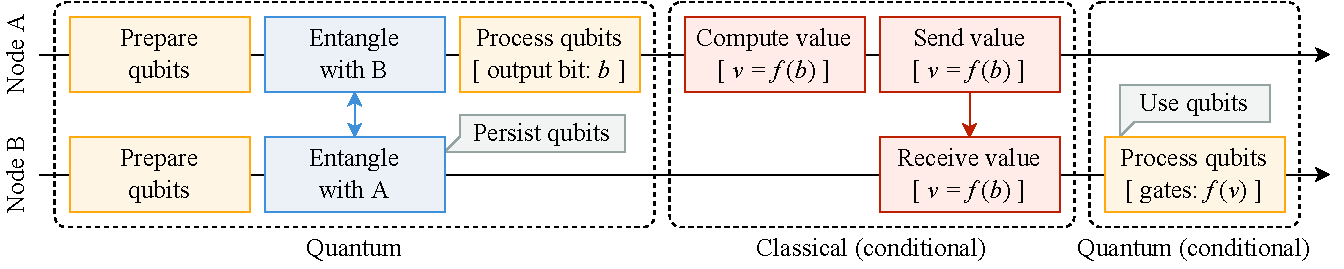
\includegraphics[width=\linewidth]{figures/app-struct.pdf}
    \caption{
        Structure of a typical quantum network application (blind quantum
        computation~\cite{broadbent_2009_ubqc, childs_2005_secure_qc}), which consists of
        interleaved quantum processing blocks and classical processing blocks. Quantum processing
        blocks include local quantum operations (gates and measurements, yellow boxes) and network
        operations (entanglement generation, blue boxes). The execution of some classical and
        quantum blocks might be conditional on classical and quantum data coming from previous
        blocks. Qubit states in quantum blocks may have to persist (``Persist qubits'') to be used
        in later quantum blocks (``Use qubits''), e.g. following the reception of classical messages
        from the remote node.
    }
    \label{fig:app-struct}
\end{figure}

Up to now, demonstrations of quantum networking beyond \acrshort{qkd} focused on hardware
realizations. Different types of end node quantum hardware have been realized, ranging from simple
photonic devices on which the only operation is a measurement~\cite{vallone_2015_satellite,
yin_2017_satellite}, to fully-fledged quantum processors with a network
interface~\cite{bernien_2013_heralded, humphreys_2018_delivery, pompili_2021_multinode,
moehring_2007_ion_traps, reiserer_2015_neutral_atoms}. The largest quantum network linking quantum
processors to date connects three nodes~\cite{pompili_2021_multinode} based on nitrogen-vacancy
centers in diamond (\acrshort{nv} centers) at the physical layer. Demonstrations of quantum
networking applications beyond \acrshort{qkd} have been performed using several photonic
devices~\cite{barz_2012_demonstration, thalacker_2019_anonymous, bozzio_2020_coin,
ng_2012_noisystorage}. Central to all these demonstrations is that the software to control the
hardware was specific to the experiment setup, written to perform one single task (the experiment
itself) and programmed into low-level control devices. In fact, often applications were not even
actually fully realized towards a user but quantum data was collected to show that the hardware is
in principle good enough for that specific application~\cite{zhang_2022_diqkd,
liu_2022_photonic_diqkd}.

In order to advance quantum networks from a physics experiment to a fully-fledged quantum network
system, we would need a combined software-hardware system that is built as a series of abstraction
layers. These abstractions should expose a simple interface for the user to write applications in
high-level, platform-independent software, and be able to interact with a variety of candidate
platforms for future quantum network hardware. When designing such a system, many challenges arise
(refer to \cref{sec:background:challenges} for details), which can be roughly classified into three
areas. First, there exist \emph{fundamental differences} between classical and quantum
communication. A example of this is the concept of heralded entanglement generation, which requires
coordinated actions by both nodes involved --- that is, the operations to produce entanglement need
to be scheduled at both nodes at the same time. Second, the \emph{technological limitations} of
near-term quantum devices impose stringent demands on the performance of such a system. One example
is that the same quantum device is used for processing as well as networking, which implies that
local operations cannot be scheduled independently of network operations --- which in turn depend on
the remote node. Finally, we remark that, unlike in the study of classical operating systems, which
take advantage of the existence of advanced computer architectures defining a specific interaction
of software and hardware, there exists \emph{no general low-level quantum processor architecture}.
Ideally, our system should be able to operate under the stringent constraints imposed by current
technological limitations, but should also not be tailored to near-term quantum devices only.

\section{Background}
\label{sec:background:background}

Here, we define some basic concepts of quantum networking hardware and performance metrics,
necessary to understand the remainder of this chapter and this thesis. We refer the reader to the
book \citetitle{nielsen_chuang_2002} by \textcite{nielsen_chuang_2002} for a general introduction to
quantum information, and to the article \citetitle{dahlberg_2019_egp} by
\textcite{dahlberg_2019_egp} for more information on quantum networking. \note{Should we include
more theory in this thesis?}

\subsection{Quantum network nodes}

Generally speaking, a quantum network node is a quantum processor (or device) with an optical
interface for external communication (entanglement). The processor can perform operations on one or
more qubits. Local quantum operations range from simple qubit
measurements~\cite{vallone_2015_satellite, yin_2017_satellite} to universal quantum
computation~\cite{bernien_2013_heralded, humphreys_2018_delivery, pompili_2021_multinode,
moehring_2007_ion_traps, reiserer_2015_neutral_atoms}. Quantum networking operations allow certain
qubits to produce entanglement with a remote node. In practice, only some types of qubits are suited
for entanglement generation --- we refer to such qubits as \emph{communication qubits} --- and only
these qubits have an optical interface to the outside world. Other types of qubits --- referred to
as \emph{storage qubits} --- are instead more suited for storing quantum states for longer times (up
to seconds in some cases~\cite{abobeih_2018_one_sec, bradley_2019_one_min}). Often, storage qubits
can also be used to process quantum information directly. On some quantum devices instead, for
instance \acrlong{nv} centers in diamond (\acrshort{nv} centers), communication qubits are also the
main gateway for local quantum gates, meaning that most processing operations need to step though
these qubits, and thus their usage needs to be shared between local quantum computation and
entanglement generation. What operations can be performed on what types of qubits depends on the
specific quantum device. We remark that, at this stage of technological development, qubits, as well
as any quantum operations applied on them, are not perfect. In fact, their quality even depends on
the specific device sample being used.

\subsection{Timing constraints}

Quantum devices are generally controlled using a variety of classical signal generators, depending
on the quantum device itself. For instance, in \acrshort{nv} centers, the quantum device is
controlled using microwave as well as laser pulses. The device-level control must satisfy hard
real-time constraints and timing precision --- nanosecond precision with sub-nanosecond jitter ---
and is realized using waveform generators, lasers, and custom electronics assisted by a dedicated
microcontroller. Entanglement generation between two nodes connected by an optical fiber also
requires the same scale of timing synchronization between the two devices~\cite{dahlberg_2019_egp,
pompili_2022_experimental}. The low-level control of other quantum platforms is realized
similarly~\cite{moehring_2007_ion_traps, reiserer_2015_neutral_atoms}. On top of those constraints,
qubits have a limited lifetime --- the states they hold must be processed before they become
invalid. On some devices, qubit lifetimes have been shown to exceed one
second~\cite{abobeih_2018_one_sec}. Nevertheless, the quality of a qubit state is not constant
throughout its lifetime, but it \emph{decoheres} (becomes worse) at a certain rate. Qubit lifetimes
and decoherence, however, are a technological limitation, rather than a fundamental one, and are
expected to become more tractable in the future.

\subsection{Performance metrics}

Next to standard classical performance metrics such as latency and throughput, the performance of
quantum networking applications hinges on the quality of the quantum execution too. In the quantum
networking domain, it is not generally an objective to eliminate all errors towards the application
level~\cite{dahlberg_2019_egp, vardoyan_2022_netarch}, and hence the performance of any operating
system for quantum network nodes would be measured by the execution quality, and by the trade-offs
with classical performance metrics~\cite{dahlberg_2019_egp, vardoyan_2022_netarch}. This quantum
quality is generally measured by the quantum \emph{fidelity} $F \in [0,1]$, where a higher value
corresponds to higher quality. For a quantum state, $F$ measures the quality with respect to an
ideal state. For a quantum gate or measurement, it measures the quality of execution, averaged over
all possible states that it could be applied to. For a specific application, $F$ can be translated
into its quantum performance.

\section{Challenges}
\label{sec:background:challenges}

Whilst the high-level goals for an operating system for quantum nodes mimic those of a classical
operating system, we face a number of general challenges inherent to (near-term) quantum network
nodes and network applications:
%
\begin{inlinelist}
    \item limited available qubits, which imposes strict limits on the processing, networking, and
          storage capabilities of networking nodes;
    \item limited qubit lifetimes, which imposes strict deadlines on how fast the data must be
          processed before it becomes useless;
    \item noisy operations, which implies that applying operations on qubits degrades the quality of
          the qubit states themselves;
    \item cross-node scheduling dependencies, meaning that the operations on one node cannot be
          scheduled independently of other nodes;
    \item interaction between classical and quantum parts of a program, which requires keeping
          quantum data alive in memory while waiting for an event to occur (e.g. a message from a
          remote network node).
\end{inlinelist}

The first three challenges are technological, that is, we expect the situation to improve with
further progress in quantum hardware development. Furthermore, to a certain extent, these issues are
common to quantum computing too, from which we can draw some inspiration for their solutions. The
fourth challenge is inherent to the nature of entanglement generation and to the physics of the
devices currently in use. Successful entanglement generation requires both nodes to execute a
network operation at the same moment in time. Moreover, at this stage of development, the same
quantum device functions as the processing unit and as the network device, and consequently local
quantum operations (such as measurements and gates) and network operations cannot be performed
simultaneously~\cite{vardoyan_2019_performance}. This limitation, however, could be mitigated by a
new quantum hardware architecture separating the devices~\cite{vardoyan_2022_netarch}. Finally, the
last challenge is a fundamental issue, as it applies to quantum network applications regardless of
technological progress. It is the last two points that fundamentally differentiate a quantum
networking node from a quantum computing system, and are the key driver for a \emph{networked}
quantum node operating system.

\printbibliography[heading=subbibintoc,title={References}]
